\documentclass{article} % This command is used to set the type of
% document you are working on such as an article, book, or presenation

\usepackage{geometry} % This package allows the editing of the page layout
\usepackage{amsmath}  % This package allows the use of a large range
\usepackage{
  minted,
  float,
  amsmath,      % Math Environments
  amssymb,      % Extended Symbols
  enumerate,        % Enumerate Environments
  graphicx,      % Include Images
  lastpage,      % Reference Lastpage
  multicol,      % Use Multi-columns
  multirow      % Use Multi-rows
}
% of mathematical formula, commands, and symbols
\usepackage{graphicx}  % This package allows the importing of images

\newcommand{\question}[2][]{
  \begin{flushleft}
    \textbf{Question #1}: \textit{#2}

\end{flushleft}}
\newcommand{\sol}{\textbf{Solution}:} %Use if you want a boldface solution line
\newcommand{\maketitletwo}[2][]{
  \begin{center}
    \Large{\textbf{Assignment #1}

    CS4375} % Name of course here
    \vspace{5pt}

    \normalsize{N. Ohayon Rozanes  % Your name here

    \today}        % Change to due date if preferred
    \vspace{15pt}

\end{center}}

\usepackage{amsmath}
\DeclareMathOperator*{\argmax}{arg\,max}
\DeclareMathOperator*{\argmin}{arg\,min}

\begin{document}
\maketitletwo[5]  % Optional argument is assignment number
%Keep a blank space between maketitletwo and \question[1]

\question[1]{Naive Bayes}
\begin{enumerate}
  \item As in the usual set up for the naive bayes, we have a collection of
    random variable tuples $(x^i, y^i)$, where each $x^i$ is i.i.d from
    some unknown underlying distribution $X$, the independent assumption
    allows us to say that $p(x^i | p^j) = p(x^i)$, that is, observations
    are pairwise independent. $y^i$ is a discrete random variable,
    taking on one out of $K$ values, denoted as $C^k$ and has some
    dependence on $x^i$. Typically, $X$ is a discrete random variable, so
    it is natural to speak about the probability $p(X = x^i)$. Using a
    well known fact from probability, if $Z$ is a continuous variables,
    then $p(Z = z^i) = 0$ almost surely. This presents an issue, in the
    naive bayes classifier since $(X | Y = C^k)$ is a continuos
    random variable, so
    $p(X = x^i | Y = C^k) = 0$  almost surely, causing the likelihood to
    be $0$ and the classifier to be undefined
    \begin{align*}
      \hat y &= \argmax_{k} p(C^k)\prod_i^n p(x^i\vert C_k)\\
      &= \argmax_{k} \{0, 0 , 0 \hdots\} \\
    \end{align*}

    We can get around this analytical issue by discretizing the predictor
    vector:
    \begin{itemize}
      \item First we would bin the observed values in whatever method is
        most representative of the predictor's nature (equal-width, quantile,
        etc.)
      \item Then we normalize the histograms by dividing the height of
        each column by $n$, we get back a discrete random variable
      \item Repeat this procedure element wise for each entry in the
        feature vector
      \item let $x_{ij}$ be the $j$th entry of the $i$th feature vector,
        we can calculate the likelihood as:
        \[
          p(x^i \vert C_k) = \prod p(x_{ij} \vert C_k)
        \]
    \end{itemize}
  \item If instead we insisted on treating the probability
    distribution of the feature vector as continuous, the other
    option is to learn the parameters of the predictor variables. To
    start with, we have to make an additional assumption regarding
    the distribution of the data; generally, assuming normally
    distributed data is a good first guess, so from the observed data
    $x^i$ we would like to find parameters $\mu$ and $\sigma^2$. Since
    the following procedure can be repeated element wise for each
    component of the feature vector, we focus on the univariate case:
    \begin{itemize}
      \item Group the data set for each class $C^k$ present in the
        data set, yielding the sets $\{x^i\}_k$
      \item The likelihood function of the normal distribution is
        described as follows:
        \[
          L(\mu, \sigma^2 \mid \{x^i\}_k) = \prod_{x^i \in \{x^i\}_k}
          f_X(x^i; \mu, \sigma^2)
        \]
        Skipping a few steps:
        \[
          L(\mu, \sigma^2 \mid \{x^i\}_k) =
          \frac{\exp\left(\frac{-1}{2\sigma^2}\sum_{x^i \in
          \{x^i\}_k}(x^i-\mu)^2\right)}{(2\pi\sigma^2)^{-n_k/2}}
        \]
      \item taking the log to obtain the log likelihood
        \[
          l(\mu, \sigma^2 \mid \{x^i\}_k) = \frac{-n_k}{2}\ln(2\pi) -
          \frac{n_k}{2}\ln(\sigma^2) - \frac{1}{2\sigma^2}\sum_{x^i
          \in \{x^i\}_k} (x^i-\mu)^2
        \]
      \item taking partials with respect to $\mu$ and $\sigma^2$, and
        setting each to zero:
        \begin{align*}
          \frac{\partial l}{\partial \mu} &=
          \frac{1}{\sigma^2}\sum_{x^i \in \{x^i\}_k}
          (x^i - \mu) = 0 \\
          &\Rightarrow \hat{\mu}_k = \frac{1}{n_k}\sum_{x^i \in \{x^i\}_k} x^i
        \end{align*}
        \begin{align*}
          \frac{\partial l}{\partial \sigma^2} &= -\frac{n_k}{2\sigma^2} +
          \frac{1}{2\sigma^4}\sum_{x^i \in \{x^i\}_k} (x^i - \mu)^2 = 0 \\
          &\Rightarrow \hat{\sigma}^2_k = \frac{1}{n_k}\sum_{x^i \in
          \{x^i\}_k} (x^i - \hat{\mu}_k)^2
        \end{align*}
    \end{itemize}
    Thus we have obtained the MLE for the parameters of the normal
    distribution for each class. Using this in place of the
    likelihood function in the discrete naive bayes classifier:
    \[
      \hat y = \argmax_{k} p(C^k)\prod_i^{n_k} f_{X_k}(x^i)\\
    \]
    This slightly dubious subtitution is justified as higher density
    in the distribution conditional on the class $k$ around $x^i$ is
    roughly equivalent to points around $x^i$ being more likely to be
    in the class $k$.
\end{enumerate}
\question[2]{Logistic Regression and Regularization}
\begin{enumerate}
  \item A logistic regression with no polynomial features and no
    regularization was trained on the UCI Machine Learning Breast
    Cancer dataset.
    The results are shown below:
    \begin{table}[H]
      \centering
      \begin{tabular}{l c c c c}
        \hline
        & Train MSE & Test MSE & Train Log-Loss & Test Log-Loss \\
        \hline
        No regularization & 0.008565 & 0.024141 & 0.032905 & 0.086804 \\
        \hline
      \end{tabular}
      \caption{Degree-1 logistic regression, no regularization.}
    \end{table}
    Although we are achieving a very low test mse and log loss, with
    about a threefold increase in test MSE and log loss, in aboslute
    terms the test metrics are still very low, so while we're mildly
    overfitting, introduction of polynomial features will help more
    clearly demonstrate overfitting.

  \item Increasing the polynomial degree with no regularization to
    induce overfitting:
    \begin{table}[H]
      \centering
      \begin{tabular}{c c c c c}
        \hline
        Degree & Train MSE & Test MSE & Train Log-Loss & Test Log-Loss \\
        \hline
        1 & 0.008565 & 0.024141 & 0.032905 & 0.086804 \\
        2 & 0.000036 & 0.053557 & 0.001205 & 0.289014 \\
        3 & 0.000001 & 0.058242 & 0.000164 & 0.350616 \\
        \hline
      \end{tabular}
      \caption{Polynomial feature expansion, no regularization.}
    \end{table}
    Here we see a much more obvious and extreme overfitting pattern.
    We proceed with regularizing the degree 2 model.

  \item Applying L2 regularization to the degree-2 model to reduce overfitting:
    \begin{table}[H]
      \centering
      \begin{tabular}{c c c c c}
        \hline
        $\lambda$ & Train MSE & Test MSE & Train Log-Loss & Test Log-Loss \\
        \hline
        0     & 0.000036 & 0.053557 & 0.001205 & 0.289014 \\
        0.001 & 0.000038 & 0.053573 & 0.001253 & 0.285320 \\
        0.01  & 0.000067 & 0.053513 & 0.001723 & 0.255896 \\
        0.1   & 0.000678 & 0.041642 & 0.006817 & 0.137470 \\
        0.5   & 0.003159 & 0.035005 & 0.018961 & 0.104101 \\
        1.0   & 0.003551 & 0.041571 & 0.017593 & 0.126519 \\
        5.0   & 0.018964 & 0.051199 & 0.058573 & 0.185327 \\
        \hline
      \end{tabular}
      \caption{L2 regularization sweep on the degree-2 polynomial model.}
    \end{table}
    We get the best balance between train and test MSE, as well as a
    global minimum of test MSE, with $\lambda =0.5$. Regularization
    requires an additional parameter to tune, but will generally
    control the amount of overfitting that a model exhibits by
    penalizing it for arbitrarily adding features that don't
    sufficiently improve predictive power.

\end{enumerate}

\question[3]{K-Means and K-Mediods Clustering}
\begin{enumerate}
  \item \textbf{K-Means} partitions the data by alternating between two steps
    until convergence: (1) assign each point to its nearest centroid, and (2)
    recompute each centroid as the mean of its assigned points.
    Formally, letting
    $\mu_k$ denote the centroid of cluster $k$ and $S_k$ its assigned set:
    \begin{align*}
      z_i &= \argmin_k \|x_i - \mu_k\| \\
      \mu_k &\leftarrow \frac{1}{|S_k|} \sum_{i \in S_k} x_i
    \end{align*}
    If a cluster becomes empty, its centroid is reinitialized to a random data
    point. The model was trained on the digits dataset ($k=10$) and evaluated
    via per-digit misclassification rate and log-loss, where cluster-to-label
    assignment is resolved by majority vote within each cluster.
    \begin{figure}[H]
      \centering
      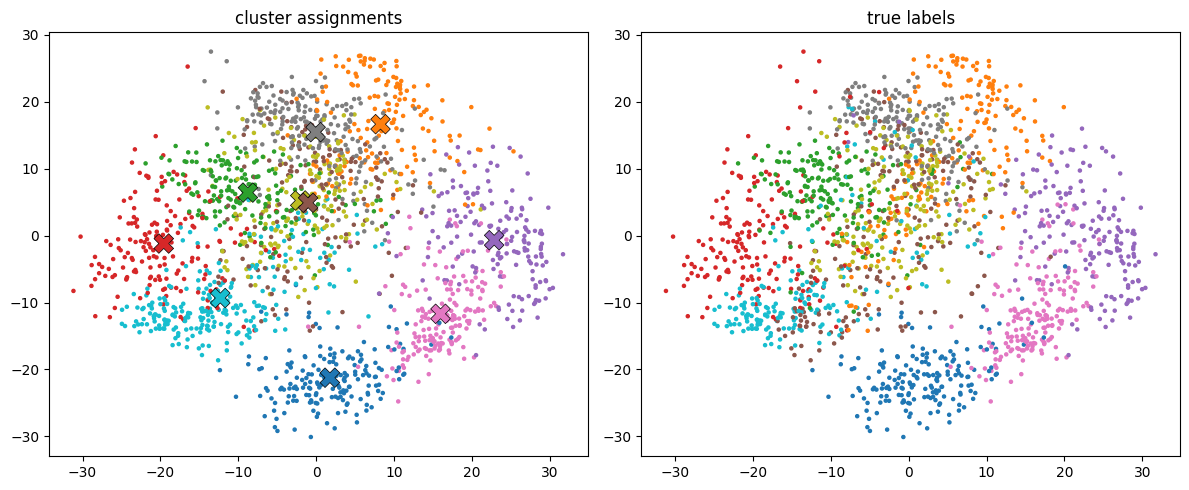
\includegraphics[width=\textwidth]{code/kmeans_clusters.png}
      \caption{K-Means cluster assignments (left) vs.\ true labels (right),
      projected onto the first two PCA components.}
    \end{figure}

  \item \textbf{K-Medoids} follows the same assign-then-update structure, but
    constrains each cluster center to be an actual data point — the
    \emph{medoid} — defined as the point minimizing the total distance to all
    others in its cluster:
    \[
      m_k = \argmin_{p \in S_k} \sum_{i \in S_k} \|x_i - p\|
    \]
    Because medoids must lie in the dataset, K-Medoids is more robust to
    outliers than K-Means; a single extreme point cannot distort the center the
    way it would when taking a mean.
    \begin{figure}[H]
      \centering
      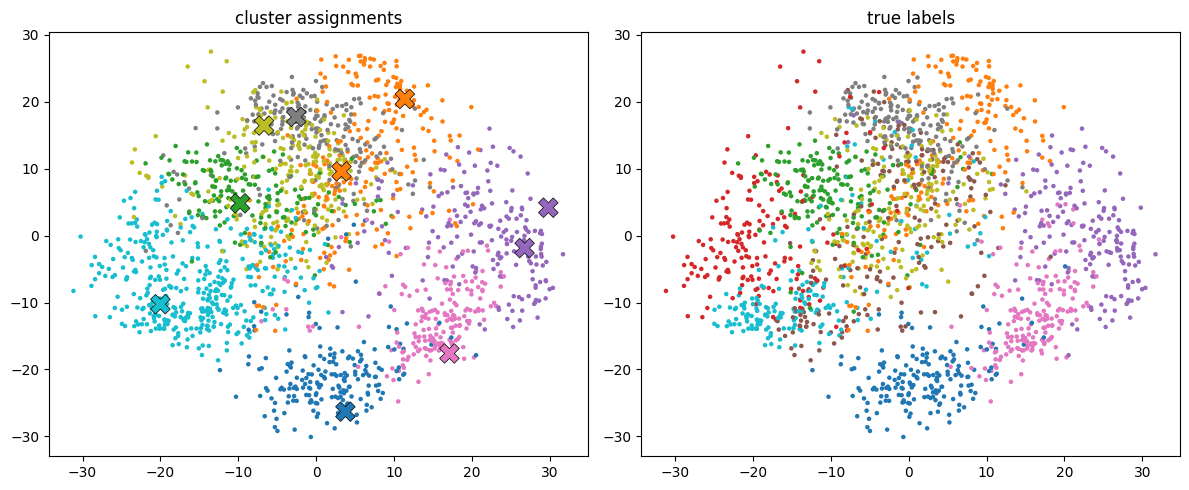
\includegraphics[width=\textwidth]{code/kmediods_clusters.png}
      \caption{K-Medoids cluster assignments (left) vs.\ true labels (right),
      projected onto the first two PCA components.}
    \end{figure}
    An issue that both K-Means and K-Mediods face is that certain
    clusters who share a particular element will cause the cluster
    for the other to collapse, further some clusters simply dominate
    cluster centers, causing 100\% cluster misidentification.
\end{enumerate}
\question[4]{Variance Bias Tradeoff}
In each of the following classifiers, we assume that $\{x^1, x^2
\hdots x^n \}$ are i.i.d random vectors in $\mathbb{R}^m$, each
of which corresponds to $\{y^1, y^2...y^N\}$ which are discrete
random variables takign on one of $\{1...C\}$ classes.
\begin{enumerate}
  \item Logistic Regression vs. Decision Trees: Given that we do not
    prune or control the max depth of the tree, it will always
    overfit, and thus will have a higher variance and low bias on the
    training set when compared on the training data. This is a result
    of the model complexity of the linear logistic regression being
    exactly determined by the data, while the unpruned desicion tree
    can grow until perfect classification has been achieved. We now
    analyze the more representative case where we limit the decision
    tree to $N$ levels:
    The logistic regression classifier (in the case where there are
    multiple classes), trains one function logit function of the following form:
    \[
      p_i(x) = \frac{1}{1+e^{-(b_i + w_i^Tx)}}
    \]
    for each class $i$, then takes the softmax between them to output
    the predicted classifier. This results in $i$ bias terms and $m *
    i$ weights a total of $i(m+1)$. On the other hand, given a max
    depth of $N$, a decision tree will have at most $2^{N+1} - 1$
    parameters, one for each node. So generally speaking, while
    \[
      i(m+1) \le 2^{N+1} - 1
    \]
    The logistic regression will have lower variance and higher bias,
    and the relation will reverse otherwise.
  \item Decision Tree vs. Random Forest vs. Gradient Boosted Tree:
    The decision tree will have the highest variance and lowest bias,
    as it will try to perfectly classify the training dataset. The
    random forest will try to lower the variance at the cost of
    increasing bias by averaging together multiple weaker
    classifiers, thereby resulting in more stable classifications
    that will generalize better but do worse on the training data
    set. The gradient boosted tree will limit the classifier at every
    step, and sequentially improve it by prioritizing on sample which
    the tree finds difficult, this results in a tree with a variance
    and bias between the base tree and the random forest.
  \item Logistic Regression vs. 1NN Classifier: The 1NN classifier
    will depend on exactly just the nearest neighbor, this results in
    a very unstable classifier, where even nearby points can be in
    completely different clusters. As such, we end up with a very
    high variance model, with bias that depends very heavily on the
    data, but will usually be somewhat low bias. The logistic
    regression will result in a much more stable, lower variance
    model, that will have a higher bias on the training set for the
    noisy labels.
  \item 5NN vs 1NN: The 5NN classifier will result in a much more
    stable classifier since its estimate is based on more neighbors,
    so small changes or noisy data will not vary the classification
    as much. For the reasons above, the 5NN classifier will have
    higher bias and lower variance.
  \item Depth 5 vs. Depth 10: The depth 10 tree will subdivide the
    data into purer and purer partitions, which results in a
    classifier which has very low bias but very high variance. The
    depth 5 tree will probably be unable to purely subdivide the
    data, resulting in a higher bias but a lower variance.
  \item Random forest 100 Trees vs 10 Trees: Recall that for any
    sample of $N$ random variable, the variance of the average is the
    variance of the variable divided by $N$: clearly, the $100$ Tree
    random forest will have lower variance than the $10$ Tree random
    forest. A similar analysis can be applied to the output of the
    averaged trees:
    \begin{align*}
      E[\frac{1}{N}\sum^{N} X] &= \frac{1}{N}\sum^{N} E[X] \\
      &= E[X]
    \end{align*}
    Thus, we would not expect the average output of the random forest
    to change that much in the long run between different values of
    $N$, so the bias remains unchanged between the two forests.
  \item Ada boost with 10 stumps vs. Ada boost with 100 stumps: In a
    boost tree, each new descision stump represents an additional
    weak classifier that is conglomerated into the model at the end.
    That is, each stump increases model complexity, therefore, the
    100 sump AdaBoost classifier will be a higher variance and lower
    bias model, compared to the 10 stump ada boost model.
  \item Linear regression vs Quadratic regression: The Quadratic
    regression introduces an additional parameter to learn in the
    optimization, that is, it is a slightly more complex model, on
    merit of that the quadratic regression will have lower bias and
    higher variance.
\end{enumerate}
\break
\question[5]{Ensemble Methods}
\begin{enumerate}
  \item The three models were trained on 100 synthetic datasets, each with
    $n=100$ samples drawn from $x \sim \mathrm{Uniform}(0,1)$ with
    $y = \sin(2\pi x) + \varepsilon$, $\varepsilon \sim \mathcal{N}(0,\,0.3^2)$.
    Predictions were evaluated on 1000 evenly spaced test points in $[0,1]$.
    The figure below shows one representative single fit alongside the mean
    prediction across all 100 fits for each model.

    \begin{figure}[H]
      \centering
      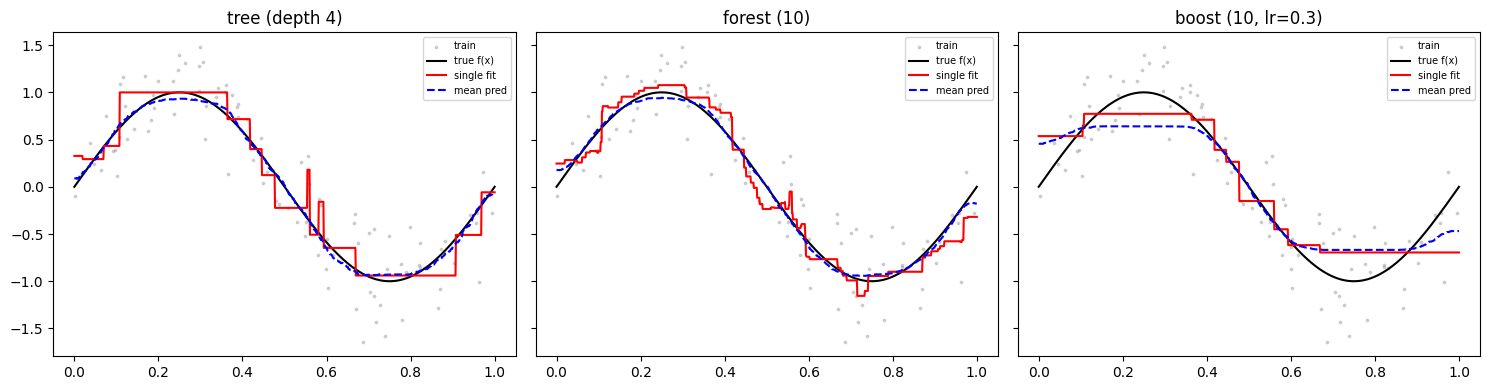
\includegraphics[width=\textwidth]{bias_variance.png}
      \caption{Representative single fit (red) and mean prediction (blue dashed)
        vs.\ the true function (black) for each model.  Gray dots are training
      points from the representative dataset.}
    \end{figure}

    The bias$^2$, variance, and MSE computed across all 100 datasets and
    averaged over the test set are:

    \begin{table}[H]
      \centering
      \begin{tabular}{l c c c}
        \hline
        Model & Bias$^2$ & Variance & MSE \\
        \hline
        Decision Tree (depth 4)       & 0.0015 & 0.0316 & 0.0331 \\
        Random Forest (10 trees)      & 0.0017 & 0.0197 & 0.0213 \\
        Gradient Boosting (10, lr=0.3) & 0.0480 & 0.0102 & 0.0582 \\
        \hline
      \end{tabular}
      \caption{Bias$^2$, variance, and MSE for each model averaged over the
      1000-point test set.}
    \end{table}

    \begin{figure}[H]
      \centering
      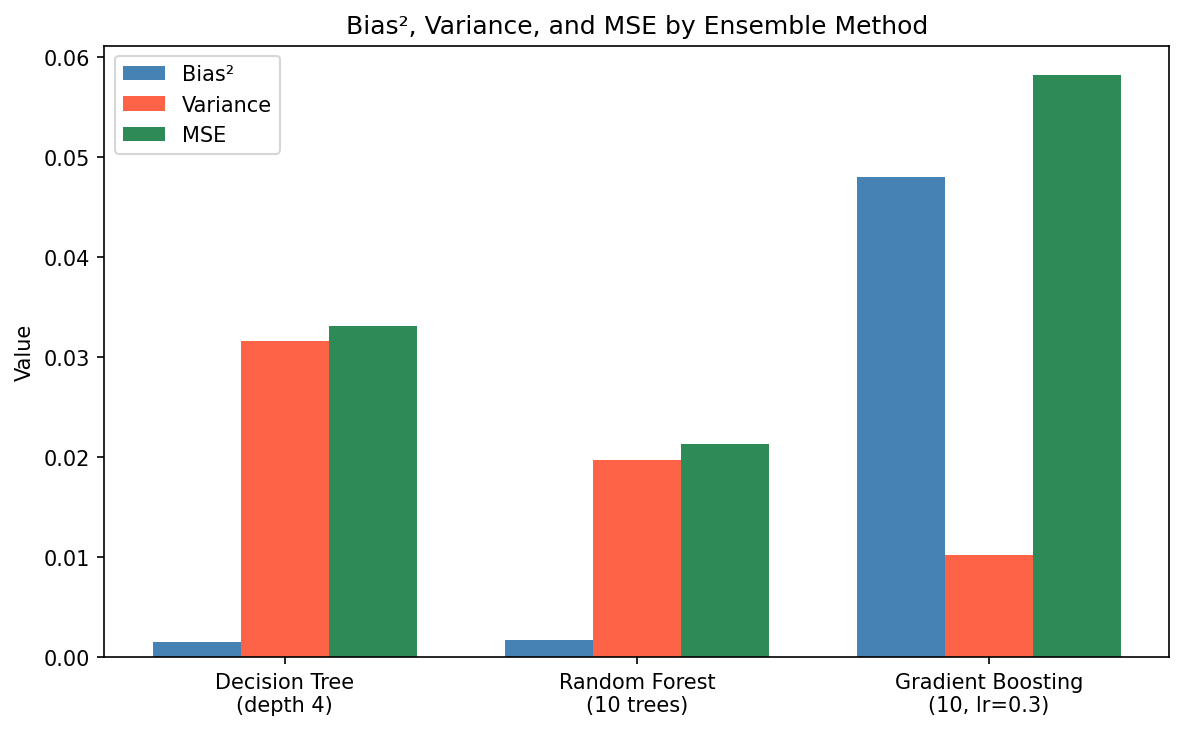
\includegraphics[width=0.85\textwidth]{code/ensemble_barplot.png}
      \caption{Bias$^2$, variance, and MSE for each ensemble method.}
    \end{figure}

  \item \textbf{Analysis.}  It's very likely that the $10$ stumps is
    simply not enough for the boosting tree to properly learn the
    residuals of the data, so it is very clearly underfitting the
    data. It follows from the BG tree underfitting that it will have
    lower variance. The random forest does show a significant
    decrease in variance compared to the decision tree, while
    maintaining a relatively low bias.

\end{enumerate}
\question[6]{Gradient Boosting}
\begin{enumerate}
  \item Logistic Loss: For $y_i \in \{0, 1\}$, and a probability $p_i
    \in  [0,1]$, which is produced by $p_i = \sigma(F(x_i))$ the
    logistic loss is given as follows:
    \[
      \phi(y_i, p_i) = y_i\ln(p_i) + (1-y_i)\ln(1-p_i)
    \]
    Since $p_i = \sigma(F(x_i))$, we first note:
    \[
      \frac{\partial p_i}{\partial F} = \frac{\partial \sigma}{\partial F}
      = \frac{e^{-F}}{(1+e^{-F})^2} =
      \sigma(F)\bigl(1-\sigma(F)\bigr) = p_i(1-p_i)
    \]
    It follows by the chain rule that
    \[
      \frac{\partial \phi}{\partial F} = \frac{\partial
      \phi}{\partial p_i}\frac{\partial p_i}{\partial F}=\left(\frac{y_i}{p_i} -
      \frac{1-y_i}{1-p_i}\right)p_i(1-p_i) = y_i - p_i
    \]
    So, the residuals:
    \[
      y'_i = p_i - y_i = \sigma(F(x_i)) - y_i
    \]
    So in every iteration, we fit a new weak (regression) tree on the $y'$ using
    the logistic loss, compute it's residuals, and add it to the list
    of trees we use to make predictions.
  \item Hinge Loss is given by, here, we do not make any stipulations
    on the way we produce $p_i$
    $$
    \phi(y_i, p_i) = \max(0, 1-y_ip_i)
    $$
    Of course, there is the rough edge at $1-y_ip_i = 0$ where the
    function is not differentiable, so we use the subgradient to get
    the residuals. Every where else, the partial derivative is:
    \[
      \frac{\partial\phi}{\partial p_i} =
      \begin{cases}
        0 & 1 > y_ip_i \\
        -y_i & 1 < y_ip_i
      \end{cases}
    \]
    At $y_ip_i = 1$, the partial is a subgradient, with any value
    $[-y_i, 0]$. So the residual is
    $$
    y_i' =
    \begin{cases}
      0 & 1 > y_ip_i \\
      y_i & 1 < y_ip_i
    \end{cases}
    $$
\end{enumerate}
\question[7]{Neural Networks}
We seek the back propagation, using
logistic loss, with ReLU activiation functions. That is, want to find

\[
  \frac{\partial \phi}{\partial W^i_{jm}}
\]
and
\[
  \frac{\partial \phi}{\partial b^i_j}
\]

First we compute the
partial of ReLU (I will be largely ignoring that ReLU is not
differentiable at $x=0$) Let
\[
  f^i(x) = \max(0, x)
\]
And at each layer $i+1$, the $j$th neuron: $x^{i+1}_j = W^i_ja^i + b^i_j$ where
$W^i_j$ is the $j$th row of the weight matrix at layer $i$ and $a^i$ is the post
activation output of the previous layer.
\[
  f^i(W^i_ja^i + b^i_j)= \max(0, W^i_ja^i + b^i_j)
\]
Then the partials are
\[
  \frac{\partial f^i}{\partial W^i_{jm}} =
  \begin{cases}
    a^i_m & W^i_ja^i + b^i_j > 0  \\
    0 & \text{otherwise}
  \end{cases}
\]
and
\[
  \frac{\partial f^i}{\partial b^i_j} =
  \begin{cases}
    1 & W^i_ja^i + b^i_j > 0  \\
    0 & \text{otherwise}
  \end{cases}
\]
From the question prior, we have that the gradient of the logistic
loss with respect to $p$ is:
\[
  \frac{\partial \phi}{\partial p} = \frac{y-p}{p(1-p)}
\]

But for the last layer the 2 dimensional vector $p$ has the form
$$
p = f^{n-1}(W^{n-1}a^{n-1} + b^{n-1})
$$

So for the $j$th output neuron:
$$
\frac{\partial \phi}{\partial W^{n-1}_{jm}} = \frac{\partial
\phi}{\partial p_j}\frac{\partial p_j}{\partial W^{n-1}_{jm}} =
\frac{y_j - p_j}{p_j(1-p_j)}
\begin{cases}
  a^{n-1}_m & W^{n-1}_j a^{n-1} + b^{n-1}_j > 0 \\
  0 & \text{otherwise}
\end{cases}
$$
and similarly for the bias:
$$
\frac{\partial \phi}{\partial b^{n-1}_j} = \frac{\partial
\phi}{\partial p_j}\frac{\partial p_j}{\partial b^{n-1}_j} =
\frac{y_j - p_j}{p_j(1-p_j)}
\begin{cases}
  1 & W^{n-1}_j a^{n-1} + b^{n-1}_j > 0 \\
  0 & \text{otherwise}
\end{cases}
$$

To calculate the next gradient, obeserve that
\[
  a^{n-1} = f^{n-2}(W^{n-2}a^{n-2} + b^{n-2})
\]

So $\phi$ is a function of $W_{jm}^{n-2}$ through both $p_1$ and
$p_2$, so by the multivariate chain rule

$$
\frac{\partial \phi}{\partial W^{n-2}_{jm}} =
\sum_k \frac{\partial \phi}{\partial p_k}
\cdot \frac{\partial p_k}{\partial a^{n-1}_j}
\cdot \frac{\partial a^{n-1}_j}{\partial W^{n-2}_{jm}} =
\sum_k \frac{y_k - p_k}{p_k(1-p_k)}\cdot W_{kj}^{n-1}
\begin{cases}
  1 & W^{n-1}_k a^{n-1} + b^{n-1}_k > 0 \\
  0 & \text{otherwise}
\end{cases}
\cdot
\begin{cases}
  a^{n-2}_m & W^{n-2}_j a^{n-2} + b^{n-2}_j > 0 \\
  0 & \text{otherwise}
\end{cases}
$$
and for the bias, the only difference is that $\frac{\partial
a^{n-1}_j}{\partial b^{n-2}_j} = (f^{n-2})'(\cdot) \cdot 1$, so the
last factor becomes $1$ instead of $a^{n-2}_m$:
$$
\frac{\partial \phi}{\partial b^{n-2}_j} =
\sum_k \frac{y_k - p_k}{p_k(1-p_k)}\cdot W_{kj}^{n-1}
\begin{cases}
  1 & W^{n-1}_k a^{n-1} + b^{n-1}_k > 0 \\
  0 & \text{otherwise}
\end{cases}
\cdot
\begin{cases}
  1 & W^{n-2}_j a^{n-2} + b^{n-2}_j > 0 \\
  0 & \text{otherwise}
\end{cases}
$$
We can generalize this arbitrarily: at each earlier layer the same
pattern repeats, accumulating one more factor of $W^l_{kj} \cdot
(f^l)'(\cdot)$ per layer stepped back, with $a^i_m$ (or $1$ for the
bias) as the final factor.

\appendix
\section*{Code}

\subsection*{Logistic Regression (\texttt{logi\_reg.py})}
\inputminted[fontsize=\small, breaklines]{python}{code/logi_reg.py}

\subsection*{K-Means (\texttt{kmeans.py})}
\inputminted[fontsize=\small, breaklines]{python}{code/kmeans.py}

\subsection*{K-Medoids (\texttt{kmediods.py})}
\inputminted[fontsize=\small, breaklines]{python}{code/kmediods.py}

\subsection*{Regression Tree / Ensemble Methods (\texttt{regresson\_tree.py})}
\inputminted[fontsize=\small, breaklines]{python}{code/regresson_tree.py}

\subsection*{Ensemble Bar Plot (\texttt{ensemble\_barplot.py})}
\inputminted[fontsize=\small, breaklines]{python}{code/ensemble_barplot.py}

\end{document}
